%%%%%%%%%%%%%%%%%%%%%%%%%%%%%%%%%%%%%%%%%%%%%%%%%%%%%%%%%%%%%%%%%%%%%%%%%
% This file is part of the LaTeX sources of the OMDoc 1.3 specifiation
% Copyright (c) 2006 Alberto Gonz\'alez Palomo
% This work is licensed by the Creative Commons Share-Alike license
% see http://creativecommons.org/licenses/by-sa/2.5/ for details
\svnInfo $Id: main.tex 8453 2009-08-04 09:58:26Z kohlhase $
\svnKeyword $HeadURL: https://svn.omdoc.org/repos/omdoc/branches/omdoc-1.3/doc/spec/projects/sentido/main.tex $
%%%%%%%%%%%%%%%%%%%%%%%%%%%%%%%%%%%%%%%%%%%%%%%%%%%%%%%%%%%%%%%%%%%%%%%%%

\section[Sentido Integrated Environment]{Sentido: an Integrated Environment for OMDoc}
\begin{project}{sentido}{http://www.matracas.org/sentido/index.en.html}
\pauthors{Alberto Gonz\'alez Palomo}
\pinstitute{Toledo, Spain\footnotemark}
\end{project}
\footnotetext{\tiny{The author is currently employed part-time in the {\activemath} project,
    developed by Saarland University and the DFKI, but this work was done on his own,
    without their supervision or support.}}

{\sentido} is an integrated environment for {\indextoo{browsing}}, {\indextoo{searching}},
and {\indextoo{editing}} collections of {\omdoc} documents.
It is implemented as an extension for the {\mozilla}/{\firefox} browsers
to avoid the biggest problems found when using {\qmath}:
the need to compile the program for installing, the batch mode of interaction
that made small corrections consume much of the author's time,
and the lack of any support for document navigation and search.

\begin{myfig}{screenshot1}{{\sentido} after indexing the OMDoc repository in the library (left) and
    loading a document from it (center and right).}
  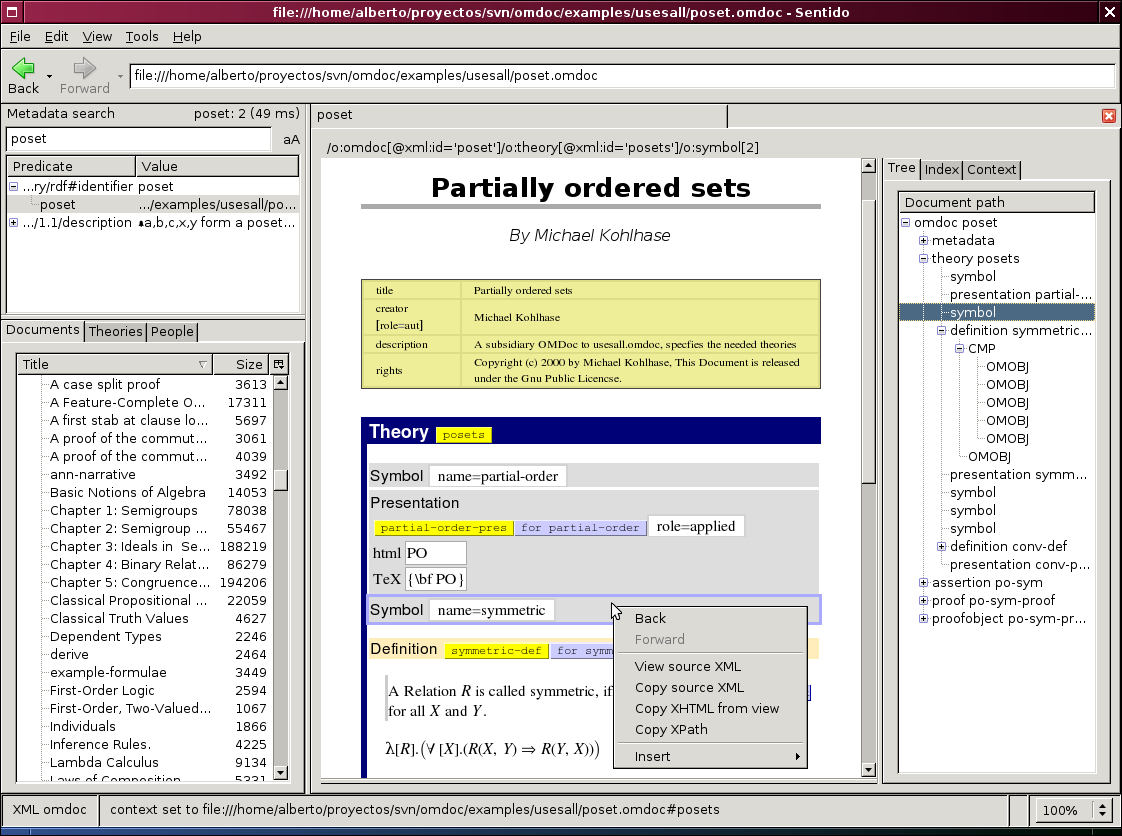
\includegraphics[width=11cm]{projects/sentido/sentido_general_poset}
\end{myfig}

{\Myfigref{screenshot1}} shows a typical session initiated by searching in the
document library (described below in more detail)
and opening one of the results.
The context menu displays the options for
browsing back and forward,
viewing the {\xml} ({\omdoc}) source of the selected element,
copying it to the {\twintoo{system}{clipboard}},
copying its {\mathml} rendering
or an {\xpath} expression that identifies it,
and inserting new elements.

\subsection{The User Interface}

The window is made to resemble the web browser,
and consists of two main panes:
the smaller one on the left contains the interface for the ``{\twintoo{document}{library}}'',
and the right one the ``{\twintoo{document}{view}}'' and associated information
like the document tree,
element identifiers index,
and context at the current cursor position.

The document library is a knowledge base about documents,
the theories defined in them,
and people mentioned in their metadata as authors, editors, translators, etc.
It is implemented as an {\rdf} store with the documents organized in
collections called ``volumes'' with references to documents,
so that different volumes can have documents in common.
The tabs labelled ``Documents'', ``Theories'' and ``People'' display
different views of the library content.

The bibliographic data for each document
is stored using the {\atwintoo{Bibliographic}{Record}{Schema}}~\cite{Lennox04},
which includes
FOAF\footnote{``Friend of a friend'', described in their web page
  \url{http://www.foaf-project.org} as being
``about creating a Web of machine-readable homepages describing people,
  the links between them and the things they create and do.''}
entries for people.

The documents in the library are indexed by the search engine,
which stores their metadata entries and theory identifiers
in an abridged inverted index to speed up the searches
to the point where ``search as you type'' becomes possible\footnote{On the
  author's 1 GHz laptop computer, the search times in a library of around two thousand
  documents are usually between 100 and 200 milliseconds.}.
The search pattern accepts regular expression syntax, as shown in {\myfigref{screenshot3}}.

\begin{myfig}{screenshot3}{Metadata Search in {\sentido}: tooltips show the content of the cropped entries.}
  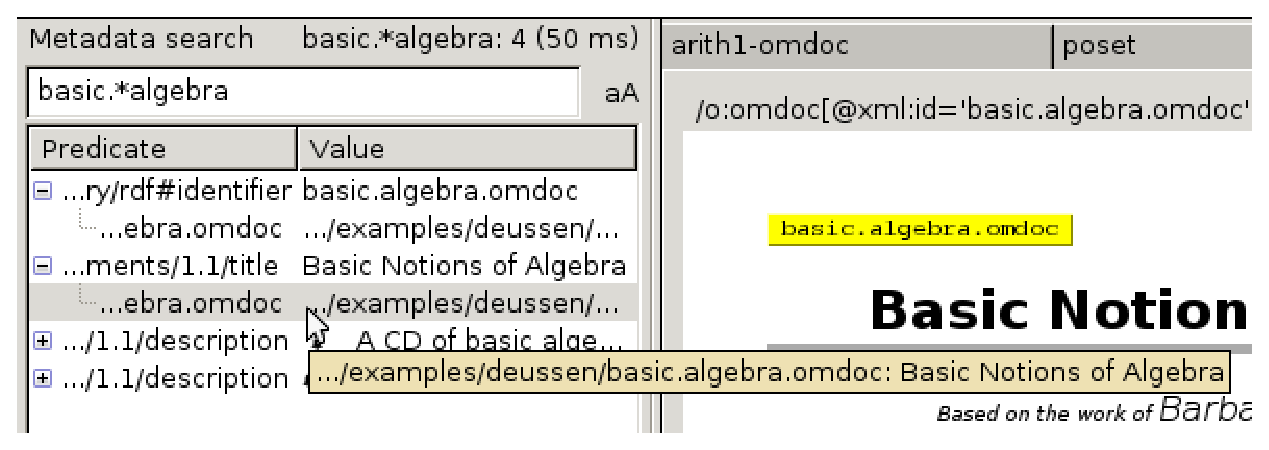
\includegraphics[width=10cm]{projects/sentido/sentido_metadata_search_tooltip_detail}
\end{myfig}

The document view is built using
{\xhtml} + {\mathml} that can be edited normally,
with the changes being propagated to the internal {\omdoc}.

The view is built on demand (using {\xslt}) as the subparts of the
document are unfolded
in the document navigation tree found in the right part of the window.
This has
been found important in practice since many real uses of {\omdoc} involve
documents that contain large lists of elements, like exercises, that are
largely independent of each other and thus do not usually require being
viewed at the same time, and the biggest delay in opening a medium to
large sized document was by far the display of the {\xhtml} view.
Another motivation for this approach is to progress towards handling the
source document more like a database, and customize its presentation
for the task at hand.

{\sentido} adds some options to the context menu in the browser,
to allow the user to open links to {\omdoc} files from web pages (see {\myfigref{screenshot2}}).

\begin{myfig}{screenshot2}{{\mozilla}'s Context Menu after Installing {\sentido}.}
  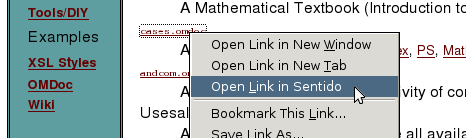
\includegraphics[width=10cm]{projects/sentido/sentido_context_menu_open_link_detail}
\end{myfig}

\subsection{Formula Editing}

Mathematical expressions are entered using a selectable linear syntax,
translated by a new version of the {\qmath} parser described in
{\mysecref{qmath}}. This is a much more capable implementation
based on {\twintoo{finite-state}{cascades}}~\cite{abney96partial}.

There are five grammars included in the install package, that are
used for translating back and forth between {\openmath} and the linear
syntax of {\qmath} and the Computer Algebra Systems
{\maxima}, {\yacas}, {\maple} and {\mathematica}.
More syntaxes can be added by writing new grammars, with a format
similar to {\qmath} ``context'' files.

\begin{myfig}{screenshot34}{The formula editor under the document view, with the input syntax menu and the text field where the formula is typed, which updates continuously the internal {\openmath} representation and the {\mathml} view.}
  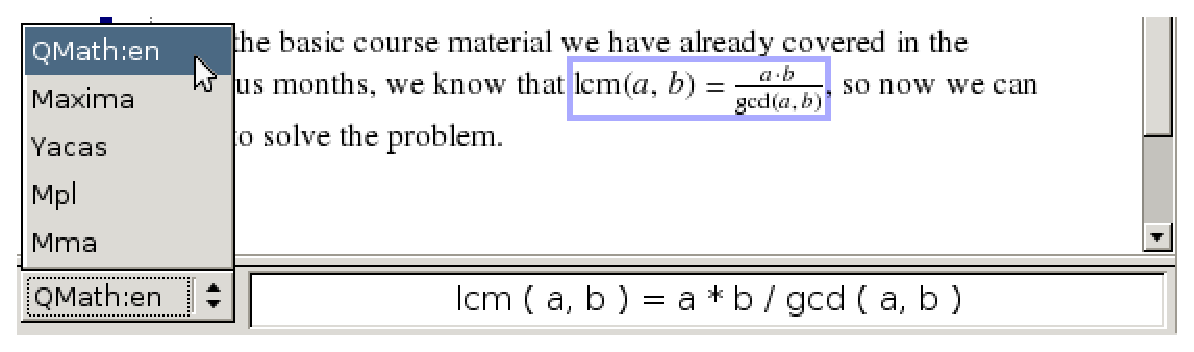
\includegraphics[width=10cm]{projects/sentido/sentido_equation_editor_QMath-en}
\end{myfig}

When the cursor enters a formula, the linear input field appears
at the bottom of the document view, as seen in {\myfigref{screenshot34}}.
It contains a text field for editing, and a menu button for
selecting the syntax, which can be done at any moment:
the linear expression is regenerated instantaneously from its {\openmath} form,
so it is possible to enter a formula using, for instance,
{\mathematica} syntax, then select another syntax such as {\maple}, and get the
expression immediately translated, going through its {\openmath} representation ({\myfigref{screenshot35}}).

\begin{myfig}{screenshot35}{The formula is translated by {\sentido} each time the user selects another syntax (left, the vertical line is the blinking caret), and it is possible to view the parse tree (right), updated as the input is modified.}
  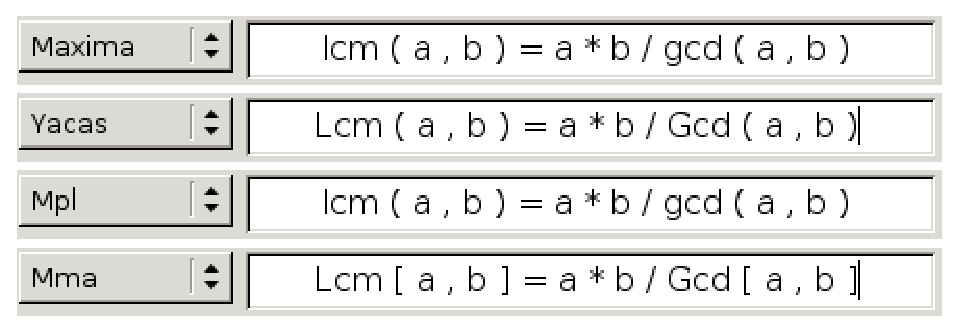
\includegraphics[width=6cm]{projects/sentido/sentido_equation_editor_Maxima_Yacas_Mpl_Mma}\quad
  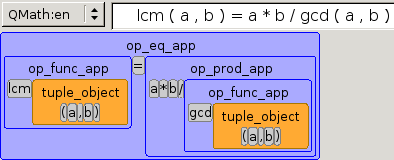
\includegraphics[width=5cm]{projects/sentido/sentido_equation_editor_parse_tree}
\end{myfig}

Insertion of formulae is achieved by typing the dollar symbol ``\$'',
which produces an empty formula readily editable so that the sequence
of keystrokes is similar to typing {\TeX} or {\qmath} text:
one can type {\verb|$e^(pi*i)+1=0$|} and get $e^{\pi i}+1=0$
without having to look at the formula editor or use the mouse.
The changes as the formula is being modified are stored,
and the display updated from the {\openmath} form,
at each point when there is a complete parse of the formula.
This gives immediate feedback on how the program understands the input.

%While it uses internally the
%same concept of ``context'' files that contain the syntax definition,
%the document author does not need to care about them explicitly any more.
An important difference is that there is no need to care about ``context files'' any more.
In {\qmath}, specifying a ``context'' had a double function: putting
symbols in scope for disambiguation, and selecting a notation style for them.
Those aspects are separated in {\sentido}:
the in-scope symbols are automatically determined from
the enclosing theory and those imported from it (recursively),
and the notation is selectable by the user.

Note that the parser allows any characters supported by the browser
rendering engine of {\mozilla}/{\firefox} (a big subset of {\unicode}),
not just ASCII. For example, the number $3.14159265...$ can be entered either
as $\pi$ or with an ASCII form depending on the selected syntax:
``pi'' for {\qmath}, ``\%pi'' for {\maxima},
or ``Pi'' for {\yacas}, {\maple} and {\mathematica}.


\subsection{Future Work and Availability}

{\sentido} is a long term personal project
that has been in development for several years (since 2004),
entirely in the author's spare time and using his own computing resources,
based on experiments\footnote{Some of those early experiments with {\mozilla}
inspired work done on adapting {\openoffice} and {\texmacs} for {\omdoc}
in collaboration with George Goguadze~\cite{GogPal:amesam03}}
and notes collected during the development of {\qmath}.
Therefore, we expect it to continue developing during the foreseeable future
unless a better application appears that makes it redundant.

Its components are designed to be reusable, which is tested from time to time by producing
spin-off applications that use subsets of its functionality in a self-contained way. One
example is the small Computer Algebra System called {\algebra}~\cite{algebra:URL}, that
contains parts of {\sentido} such as the new parser combined with specific ones like the
function plotter and the term rewriting engine.

Future developments will focus on what we consider the two main tasks for a development
environment for semantic encoding of mathematical content:
\begin{itemize}
\item Ease the tedium of writing all the details needed for an unambiguous encoding of the
  content.  This is where the flexible input parser comes into play: having a syntax
  redefinable at any point in the content simplifies the expression input, as the syntax
  can be adapted to the context in which an expression occurs.
\item Provide some benefit once we have the semantic encoding which would not be present
  with an ambiguous encoding such as {\TeX}.  Here we need to implement detailed checking
  and strong search capabilities.  A next step would be to assist the writing process by
  inferring new content and informing the input interface about the context as mentioned
  above.
\end{itemize}

Some planned improvements in {\sentido} are:
\begin{itemize}
\item Make the browser open {\omdoc} documents linked from normal pages directly in
  {\sentido}, by implementing a stream handler for the {\tt{MIME}} type
  {\tt{application/omdoc+xml}}.
\item Integrate {\algebra} into {\sentido}, to add automated symbolic manipulation to the
  document editing process.
\item Extend the checking being done on the theories: at the time of writing these lines,
  only the theory import relations are checked for loops and unknown theory references,
  which was already enough to locate several mistyped theory identifiers in the {\omdoc}
  repository.
\item Implement useful features found in other projects such as
  {\theorema}~\cite{piroi04environment}.  This is strongly related to the two points above
  since {\theorema} implements many features needed for the task of content checking which
  are still missing in {\sentido}, and some of them are available in proof-of-concept form
  in {\algebra}.
\end{itemize}

{\sentido} is Free Software distributed under the GNU General Public License
(GPL~\cite{GPL}).

%%% Local Variables: 
%%% mode: latex
%%% TeX-master: "../../omdoc"
%%% End: 


% LocalWords:  Sentido sentido Gonz alez Palomo screenshot FOAF metadata GHz
% LocalWords:  tooltips subparts qmath syntaxes Goguadze omdoc GPL sentido
% LocalWords:  sentido sentido
